\section{Tên sách - Lớp 1x - Ôn tập giữa học kì 1 - Đề y}
\caulc
\Opensolutionfile{ans}[ans-ABCD]
\begin{ex}%[1D1H2-2]%[KNTT - Lớp 11 - Ôn tập giữa học kì 1 - Đề 3]%[Phúc Hậu]
	Cho góc lượng giác $\alpha$ thỏa mãn $\cos \alpha=-\dfrac{3}{4}$ và $\dfrac{\pi}{2}<\alpha<\pi$. Tính $\sin \alpha$.
	\choice
	{$\sin \alpha=\dfrac{-\sqrt{7}}{4}$}
	{$\sin \alpha=\dfrac{1}{4}$}
	{\True $\sin \alpha=\dfrac{\sqrt{7}}{4}$}
	{$\sin \alpha=-\dfrac{1}{4}$}
	\loigiai{
	Do $\dfrac{\pi}{2}<\alpha<\pi$ nên $\sin \alpha=\sqrt{1-\cos ^{2}\alpha}=\dfrac{\sqrt{7}}{4}$.
}
\end{ex}

\begin{ex}%Câu 2%[1D1N3-3]%[KNTT - Lớp 11 - Ôn tập giữa học kì 1 - Đề 3]%[Phúc Hậu]
	Chọn khẳng định đúng.
	\choice
	{$\cos2a=\sin^2 a-\cos^2 a$}
	{$\cos2a=2 \sin^2 a+1$}
	{\True $\cos2a=2 \cos^2 a-1$}
	{$\cos2a=1-2 \cos^2 a$}
	\loigiai{	
	Ta có $\cos 2 a=\cos ^{2}a-\sin ^{2}a=2 \cos ^{2}a-1=1-2 \sin ^{2}a$.
}
\end{ex}

\begin{ex}%Câu 3%[1D1H4-5]%[KNTT - Lớp 11 - Ôn tập giữa học kì 1 - Đề 3]%[Phúc Hậu]
	Tìm chu kì $T$ của hàm số $y=\tan (5 \pi x)$.
	\choice
	{$T=\dfrac{\pi}{5}$}
	{$T=\dfrac{2}{5}$}
	{$T=\dfrac{2 \pi}{5}$}
	{\True $T=\dfrac{1}{5}$}
	\loigiai{
		Hàm số $y=\tan (a x+b)$ tuần hoàn với chu kì $T=\dfrac{\pi}{|a|}$.\\
		Áp dụng: Hàm số $y=\tan (5 \pi x)$ tuần hoàn với chu kì $T=\dfrac{1}{5}$.
}
\end{ex}

\begin{ex}%Câu 4%[1D1N5-3]%[KNTT - Lớp 11 - Ôn tập giữa học kì 1 - Đề 3]%[Phúc Hậu]
	Giải phương trình $\cos x=-\dfrac{1}{2}$.
	\choice
	{\True $x= \pm \dfrac{2 \pi}{3}+k 2 \pi,\,k\in\mathbb{Z}$}
	{$x= \pm \dfrac{\pi}{6}+k \pi,\,k\in\mathbb{Z}$}
	{$x= \pm \dfrac{\pi}{3}+k 2 \pi,\,k\in\mathbb{Z}$}
	{$x= \pm \dfrac{\pi}{6}+k 2 \pi,\,k\in\mathbb{Z}$}
	\loigiai{
	Ta có	$\cos x=-\dfrac{1}{2}\Leftrightarrow \cos x=\cos \dfrac{2 \pi}{3}\Leftrightarrow x= \pm \dfrac{2 \pi}{3}+k 2 \pi,\, k \in \mathbb{Z}$.
}
\end{ex}

\begin{ex}%Câu 5%[1D1H5-3][KNTT - Lớp 11 - Ôn tập giữa học kì 1 - Đề 3]%[Phúc Hậu]
	Giải phương trình $\sin x=\dfrac{1}{2}$ trên đoạn $\left[-\dfrac{\pi}{2}; \dfrac{\pi}{2}\right]$.
	\choice
	{$x=\dfrac{5 \pi}{6}$}
	{$x=\dfrac{\pi}{3}$}
	{$x=\dfrac{\pi}{2}$}
	{\True $x=\dfrac{\pi}{6}$}
	\loigiai{
	Ta có $\sin x=\dfrac{1}{2}\Leftrightarrow\hoac{&x=\dfrac{\pi}{6}+2 k \pi \\& x=\dfrac{5 \pi}{6}+2 k \pi }(k \in \mathbb{Z})$. \\
	Vì $x \in\left[-\dfrac{\pi}{2}; \dfrac{\pi}{2}\right]$ nên $x=\dfrac{\pi}{6}$.
}
\end{ex}

\begin{ex}%Câu 6%[1D2N1-3]%[KNTT - Lớp 11 - Ôn tập giữa học kì 1 - Đề 3]%[Phúc Hậu]
	Cho dãy số $\left(u_{n}\right)$ với $u_{n}=1-\dfrac{1}{n+1}$. Tìm tổng của hai số hạng đầu.
	\choice
	{$\dfrac{1}{2}$}
	{$\dfrac{2}{3}$}
	{$\dfrac{4}{5}$}
	{\True $\dfrac{7}{6}$}
	\loigiai{	
	Ta có $u_{1}=1-\dfrac{1}{2}=\dfrac{1}{2}$; $u_{2}=1-\dfrac{1}{3}=\dfrac{2}{3}$.\\
	Vậy $u_{1}+u_{2}=\dfrac{1}{2}+\dfrac{2}{3}=\dfrac{7}{6}$.
}
\end{ex}

\begin{ex}%Câu 7%[1D2N2-4]%[KNTT - Lớp 11 - Ôn tập giữa học kì 1 - Đề 3]%[Phúc Hậu]
	Cho cấp số cộng $\left(u_{n}\right)$ có số hạng đầu $u_{1}=-2$ và công sai $d=\dfrac{1}{2}$. Tính giá trị của $u_{5}$.
	\choice
	{\True $0$}
	{$-\dfrac{1}{2}$}
	{$\dfrac{1}{2}$}
	{$1$}
	\loigiai{		
		Ta có $u_{5}=u_{1}+4 d=-2+4 \cdot \dfrac{1}{2}=0$.
}
\end{ex}

\begin{ex}%Câu 8%[1D2N3-4]%[KNTT - Lớp 11 - Ôn tập giữa học kì 1 - Đề 3]%[Phúc Hậu]
	Cho cấp số nhân $\left(v_{n}\right)$ có số hạng đầu $v_{1}=\dfrac{3}{2}$ và công bội $q=4$. Giá trị của $v_{3}$ là
	\choice
	{$\dfrac{19}{2}$}
	{$\dfrac{27}{2}$}
	{\True $24$}
	{$144$}
	\loigiai{	
	Ta có $v_{3}=v_{1}\cdot q^{2}=\dfrac{3}{2}\cdot 16=24$.
}
\end{ex}

\begin{ex}%Câu 9%[1D2H3-6]%[KNTT - Lớp 11 - Ôn tập giữa học kì 1 - Đề 3]%[Phúc Hậu]
	Cho cấp số nhân $\left(u_n\right)\colon \heva{&u_1=8 \\&u_{n+1}=-\dfrac{u_n}{2}}$. Tổng $4$ số hạng đầu tiên của cấp số nhân này có giá trị là
	\choice
	{\True $5$}
	{$15$}
	{$-5$}
	{$-15$}
	\loigiai{		
	Do $u_{n+1}=-\dfrac{u_n}{2}$ nên $q=-\dfrac{1}{2}$. Khi đó $S_4=u_1\cdot \dfrac{1-q^4}{1-q}=8 \cdot \dfrac{1-\left(-\dfrac{1}{2}\right)^{4}}{1-\left(-\dfrac{1}{2}\right)}=5$.
}
\end{ex}

\begin{ex}%Câu 10%[1D5N1-2]%[KNTT - Lớp 11 - Ôn tập giữa học kì 1 - Đề 3]%[Phúc Hậu]
	Cho mẫu số liệu về ngày sinh của tất cả học sinh lớp 11A1 dưới dạng bảng sau đây
		\begin{center}
		\begin{tabular}{|l|c|c|c|c|c|c|}
			\hline
			Ngày sinh & $[1 ; 6)$ & $[6 ; 11)$ & $[11 ; 16)$ & $[16 ; 21)$ & $[21 ; 26)$ & $[26 ; 31]$ \\
			\hline
			Số học sinh & $5$ & $7$ & $6$ & $4$ & $10$ & $8$ \\
			\hline
		\end{tabular}
	\end{center}
	Mẫu số liệu trên có cỡ mẫu là bao nhiêu?
	\choice
	{\True $40$}
	{$31$}
	{$6$}
	{$5$}
	\loigiai{	
		Mẫu số liệu trên có cỡ mẫu là $5+7+6+4+10+8=40$.
}
\end{ex}

\begin{ex}%Câu 11%[1D5N1-3]%[KNTT - Lớp 11 - Ôn tập giữa học kì 1 - Đề 3]%[Phúc Hậu]
	Độ tuổi của dân cư ở một khu phố được cho bởi bảng sau
	\begin{center}
		\begin{tabular}{|c|c|c|c|c|c|c|}
			\hline
			tuổi Độ &$[20;30)$ & $[30;40)$ & $[40;50)$ & $[50;60)$ & $[60;70)$ & $[70;80]$ \\
			\hline
			Số cư dân & $25$ & $20$ & $20$ & $14$ & $15$ & $7$ \\
			\hline
		\end{tabular}
	\end{center}
	Tính độ tuổi trung bình của dân cư ở khu phố đó? (Quy tròn đến hàng phần chục).
	\choice
	{$44$}
	{\True $44{,}5$}
	{$44{,}51$}
	{$44{,}6$}
	\loigiai{	
	Ta có bảng các giá trị đại diện cho các lớp như sau:
		\begin{center}
			\begin{tabular}{|l|c|c|c|c|c|c|}
				\hline
				Độ tuối & $[20 ; 30)$ & $[30 ; 40)$ & $[40 ; 50)$ & $[50 ; 60)$ & $[60 ; 70)$ & $[70 ; 80]$ \\
				\hline
				GT đại diện & $25$ & $35$ & $45$ & $55$ & $65$ & $75$ \\
				\hline
				Số cư dân & $25$ & $20$ & $20$ & $14$ & $15$ & $7$ \\
				\hline
			\end{tabular}
		\end{center}
		Cỡ mẫu là $25+20+20+14+15+7=101$.\\
		Độ tuổi trung bình là
		\[
		\overline{x}=\dfrac{25\cdot25+35\cdot20+45\cdot20+55\cdot14+65\cdot15+75\cdot7}{101}\approx 44{,}5.
		\]}
\end{ex}

\begin{ex}%Câu 12%[1D5H2-2]%[KNTT - Lớp 11 - Ôn tập giữa học kì 1 - Đề 3]%[Phúc Hậu]
	Độ tuổi của dân cư ở một khu phố được cho bởi bảng sau:
	\begin{center}
		\begin{tabular}{|l|c|c|c|c|c|c|}
			\hline
			Độ tuổi & $[20 ; 30)$ & $[30 ; 40)$ & $[40 ; 50)$ & $[50 ; 60)$ & $[60 ; 70)$ & $[70 ; 80]$ \\
			\hline
			Số cư dân & $25$ & $20$ & $19$ & $14$ & $15$ & $7$ \\
			\hline
		\end{tabular}
	\end{center}
	Tính trung vị của mẫu số liệu trên? (Quy tròn đến hàng phần chục).
	\choice
	{$44$}
	{\True $42{,}6$}
	{$42{,}5$}
	{$44{,}6$}
	\loigiai{
		Mẫu số liệu trên có cỡ mẫu là $25+20+19+14+15+7=100$.\\
		Gọi $x_{1}$, $\ldots$, $x_{100}$ lần lượt là độ tuổi của $100$ dân cư ở khu phố trên và giả sử dãy này đã được sắp xếp theo thứ tự tăng dần. Khi đó trung vị là $\dfrac{x_{50}+x_{51}}{2}$, và hai giá trị này thuộc nhóm $[40;50)$ nên nhóm này chứa trung vị. Do đó\\
		$p=3$, $a_3=40$, $a_4=50$, $m_3=19$, $m_1+m_2=25+20=45$, $a_4-a_3=50-40=10$.\\
		Nên trung vị là $M_{e}=40+\dfrac{\dfrac{100}{2}-45}{19}\cdot 10 \approx 42{,}6$.
}
\end{ex}
\Closesolutionfile{ans}
\indapan{6}{ans-ABCD}

\cauds
\Opensolutionfile{ans}[ans-DS]
%Câu 1. 
\begin{ex}%Câu 1%[1D1H5-3]%[KNTT - Lớp 11 - Ôn tập giữa học kì 1 - Đề 3]%[Phúc Hậu]
	Cho $\cot x=-3$, $\dfrac{3 \pi}{2}<x<2 \pi$.
	\choiceTF[t]
	{\True $\tan x=-\dfrac{1}{3}$}
	{$\cos \left(\dfrac{\pi}{3}+x\right)=\dfrac{\sqrt{5}-2 \sqrt{3}}{6}$}
	{$\sin 2 x=\dfrac{4}{5}$}
	{\True $A=\dfrac{3\sin x-2\cos x}{2\sin x+\cos x}=-9$}
\loigiai{
	\begin{itemchoice}
	\itemch \textbf{Đúng.}\\
	Ta có $\tan x=\dfrac{1}{\cot x}=-\dfrac{1}{3}$.
	\itemch \textbf{Sai.}\\
	Ta có $\dfrac{1}{\sin^2 x}=1+\cot^2 x=1+(-3)^2=10 \Rightarrow \sin^2 x=\dfrac{1}{10} \Rightarrow \sin x= \pm \dfrac{\sqrt{10}}{10}$.\\
	Vì $\dfrac{3 \pi}{2}<x<2 \pi$ nên $\sin x<0$. Do đó $\sin x=-\dfrac{\sqrt{10}}{10}$.\\
	Ta có $\cos x=\cot x \cdot \sin x=-3 \cdot\left(-\dfrac{\sqrt{10}}{10}\right)=\dfrac{3 \sqrt{10}}{10}$.\\
	Vậy $\cos \left(\dfrac{\pi}{3}+x\right)=\cos \dfrac{\pi}{3} \cos x-\sin \dfrac{\pi}{3} \sin x=\dfrac{1}{2} \cdot \dfrac{3 \sqrt{10}}{10}-\dfrac{\sqrt{3}}{2} \cdot\left(-\dfrac{\sqrt{10}}{10}\right)=\dfrac{\sqrt{10}\left(3+\sqrt{3}\right)}{20}$.\\
	\itemch \textbf{Sai.}\\
	Ta có $\sin 2 x=2 \sin x \cos x=2 \cdot\left(-\dfrac{\sqrt{10}}{10}\right) \cdot \dfrac{3 \sqrt{10}}{10}=-\dfrac{3}{5}$.
	\itemch \textbf{Đúng.}\\
	$A=\dfrac{3 \sin x-2 \cos x}{2 \sin x+\cos x}=\dfrac{3 \cdot \dfrac{\sin x}{\sin x}-2 \cdot \dfrac{\cos x}{\sin x}}{2 \cdot \dfrac{\sin x}{\sin x}+\dfrac{\cos x}{\sin x}}=\dfrac{3-2 \cot x}{2+\cot x}=\dfrac{3-2\cdot(-3)}{2-3}=-9$.
\end{itemchoice}
}
\end{ex}
%Câu 2. 
\begin{ex}%[1D1V4-6]%[KNTT - Lớp 11 - Ôn tập giữa học kì 1 - Đề 3]%[Phúc Hậu]
	Cho hàm số lượng giác $f(x)=2 \cos \left(2 x+\dfrac{\pi}{6}\right)-\sqrt{3}$.
	\choiceTF[t]
	{Hàm số $f(x)$ tuần hoàn với chu kì $2 \pi$}
	{\True Phương trình $f(x)=0$ có nghiệm là $x=k \pi,~(k \in \mathbb{Z})$ và $x=-\dfrac{\pi}{6}+k \pi,~(k \in \mathbb{Z})$}
	{\True Tập xác định của hàm số là $\mathbb{R}$}
	{Giá trị nhỏ nhất của hàm số $f(x)$ trên $\left[-\dfrac{\pi}{12} ; \dfrac{\pi}{6}\right]$ bằng $2-\sqrt{3}$}
\loigiai{
	\begin{itemchoice}
	\itemch \textbf{Sai.}\\
	Chu kì tuần hoàn của hàm số là $T=\dfrac{2 \pi}{2}=\pi$.
	\itemch \textbf{Đúng.}\\
	Ta có
	\allowdisplaybreaks
	\begin{eqnarray*}
		& & 2 \cos \left(2 x+\dfrac{\pi}{6}\right)-\sqrt{3}=0 \\
		&\Leftrightarrow& \cos \left(2 x+\dfrac{\pi}{6}\right)=\dfrac{\sqrt{3}}{2}\\
		&\Leftrightarrow& \hoac{&2 x+\dfrac{\pi}{6}=\dfrac{\pi}{6}+k2 \pi \\&2 x+\dfrac{\pi}{6}=-\dfrac{\pi}{6}+k 2 \pi},\, k \in \mathbb{Z} \\
		&\Leftrightarrow& \hoac{&x=k \pi \\&x=-\dfrac{\pi}{6}+k \pi},\, k \in \mathbb{Z}.
	\end{eqnarray*}
	\itemch \textbf{Đúng.}\\
	Tập xác định của hàm số là $\mathbb{R}$.
	\itemch \textbf{Sai.}\\
	Ta có $-\dfrac{\pi}{12} \leq x \leq \dfrac{\pi}{6} \Leftrightarrow-\dfrac{\pi}{6} \leq 2 x \leq \dfrac{\pi}{3} \Leftrightarrow 0 \leq 2 x+\dfrac{\pi}{6} \leq \dfrac{\pi}{2}$.\\
	Do đó $0 \leq \cos \left(2 x+\dfrac{\pi}{6}\right) \leq 1 \Leftrightarrow-\sqrt{3} \leq 2 \cos \left(2 x+\dfrac{\pi}{6}\right)-\sqrt{3} \leq 2-\sqrt{3}$.\\
	Vậy giá trị nhỏ nhất của hàm số trên đoạn $\left[-\dfrac{\pi}{12} ; \dfrac{\pi}{6}\right]$ bằng $-\sqrt{3}$.
\end{itemchoice}
}
\end{ex}
%Câu 3. 
\begin{ex}%[1D2H3-6]%[KNTT - Lớp 11 - Ôn tập giữa học kì 1 - Đề 3]%[Phúc Hậu]
	Cho cấp số nhân $\left(u_n\right)$ với $\heva{&u_1=3 \\&u_{n+1}=5 u_n}\left(\forall n \in \mathbb{N}^*\right)$.
	\choiceTF[t]
	{\True Số hạng đầu và công bội của cấp số nhân là $u_1=3$, $q=5$}
	{Số hạng thứ $7$ của cấp số nhân là $u_7=46\,857$}
	{\True Số $29\,296\,875$ là số hạng thứ $11$ của cấp số nhân}
	{\True $M=u_4+u_5+u_6+u_7+u_8+u_9=1\,464\,750$}
\loigiai{
	\begin{itemchoice}
	\itemch \textbf{Đúng.}\\
	Ta có $u_1=3$, $u_{n+1}=5 u_n$, khi đó $\left(u_n\right)$ là cấp số nhân có số hạng đầu là $u_1=3$, công bội là $q=5$.
	\itemch \textbf{Sai.}\\
	Số hạng thứ $7$ của cấp số nhân là $u_7=u_1 \cdot q^6=3 \cdot 5^6=46\,875$.
	\itemch \textbf{Đúng.}\\
	Giả sử $u_n=29\,296\,875$. Khi đó
	\allowdisplaybreaks
	\begin{eqnarray*}
	&& u_n=29\,296\,875 \\
	&\Leftrightarrow& u_1\cdot q^{n-1}=29\,296\,875 \\
	&\Leftrightarrow& 3\cdot5^{n-1}=29\,296\,875 \\
	& \Leftrightarrow& 5^{n-1}=29\,296\,875\\
	& \Leftrightarrow& 5^{n-1}=5^{10} \\
	&\Leftrightarrow& n=11.
	\end{eqnarray*}
	\itemch \textbf{Đúng.}\\
	Ta có
	\begin{align*}
		M&=u_4+u_5+u_6+u_7+u_8+u_9\\
		&=S_9-S_3\\
	&=u_1 \dfrac{1-q^9}{1-q}-u_1 \dfrac{1-q^3}{1-q}\\
	&=3 \cdot \dfrac{1-5^9}{1-5}-3 \dfrac{1-5^3}{1-5}=1\,464\,750.
	\end{align*}
\end{itemchoice}
}
\end{ex}
%Câu 4. 
\begin{ex}%[1D5H2-3]%[KNTT - Lớp 11 - Ôn tập giữa học kì 1 - Đề 3]%[Phúc Hậu]
	Cho mẫu số liệu về cân nặng của các em học sinh trong lớp 10A đã ghép nhóm dưới dạng bảng tần số như sau:
\begin{center}
	\begin{tabular}{|l|c|c|c|c|c|c|}
		\hline
		Nhóm & $[30 ; 40)$ & $[40 ; 50)$ & $[50 ; 60)$ & $[60 ; 70)$ & $[70 ; 80)$ & $[80 ; 90)$ \\
		\hline
		Tần số & 2 & 10 & 16 & 8 & 2 & 2 \\
		\hline
	\end{tabular}
\end{center}
\choiceTF[t]
	{Cỡ của mẫu số liệu là $n=42$}
	{\True Số trung bình của mẫu số liệu trên là $56$}
	{\True Trung vị của mẫu số liệu đã cho bằng $55$}
	{Hiệu của tứ phân vị thứ ba và thứ nhất là $14$}
\loigiai{
	\begin{itemchoice}
	\itemch \textbf{Sai.}\\
	Từ mẫu số liệu ghép nhóm, cỡ của mẫu số liệu là $n=40$.\\
	\itemch \textbf{Đúng.}\\
	Từ đề bài, số trung bình của mẫu số liệu ghép nhóm:\\
	$$\overline{x}=\dfrac{35 \times 2+45 \times 10+55 \times 16+65 \times 8+75 \times 2+85 \times 2}{40}=56.$$
	\itemch \textbf{Đúng.}\\
	Từ đề bài, đầu mút trái là $50$, độ dài của nhóm là $10$, tần số của nhóm chứa trung vị là $16$.\\
	Ta có $n_m=16$; $C_2=2+10=12$; $u_m=50$; $u_{n+1}=60$.\\
	Trung vị của mẫu số liệu đó là $Q_2=M_e=50+\dfrac{\dfrac{40}{2}-12}{16} \cdot(60-50)=55$.
	\itemch \textbf{Sai.}\\
	Tứ phân vị thứ nhất của mẫu số liệu là $Q_{1}=40+\dfrac{\dfrac{40}{4}-2}{10} \cdot(50-40)=48$.\\
	Tứ phân vị thứ ba của mẫu số liệu là $Q_{3}=60+\dfrac{\dfrac{3 \cdot 40}{4}-(2+10+16)}{8} \cdot(70-60)=62{,}5$ nên hiệu của tứ phân vị thứ 3 và tứ phân vị thứ nhất là $14{,}5$.
\end{itemchoice}
}
\end{ex}
\Closesolutionfile{ans}
\indapan{3}{ans-DS}

\caukq
\Opensolutionfile{ans}[ans-KQ]
\begin{ex}%[1D1V1-4]%[KNTT - Lớp 11 - Ôn tập giữa học kì 1 - Đề 3]%[Phúc Hậu]
	Bánh xe của người đi xe đạp quay được $10$ vòng trong $5$ giây. Tính độ dài quãng đường mà người đi xe đã đi được trong $2$ phút, biết rằng đường kính của bánh xe đạp là $0{,}7$ m.
	\shortans{$528$}
	\loigiai{
	Chu vi bánh xe là $C=R \cdot 2 \pi=0{,}7\cdot3{,}14$ (m).\\
	Trong 1 giây bánh xe quay được số vòng $\dfrac{10}{5}=2$.\\
	Số vòng bánh xe quay được trong $2$ phút là $120\cdot2=240$.\\
	Vậy quãng đường mà người đi xe đã đi được trong $2$ phút là $S=0{,}7\cdot 3{,}14\cdot240 \approx 528$ (m).
}
\end{ex}

\begin{ex}%[1D1V5-6][KNTT - Lớp 11 - Ôn tập giữa học kì 1 - Đề 3]%[Phúc Hậu]
	Một cái cổng vào một trung tâm thương mại có hình dạng là một phần của đồ thị hàm số $y=2 \cos \left(\dfrac{x}{2}\right)+2$. Gọi $A$, $B$ là hai điểm nằm trên cổng và $C$, $D$ là hai điểm nằm trên mặt nền của cổng sao cho $ABCD$ là hình chữ nhật. Người quản lí trung tâm thương mại muốn lắp một cái cửa kính tự động vào hình chữ nhật $ABCD$. Tính diện tích của cái cửa cần lắp biết chiều cao của cái cửa là $AD=3$ mét.
	\shortans{$12{,}6$}
	\loigiai{	
	Chọn hệ trục tọa độ như hình vẽ:
	\begin{center}
		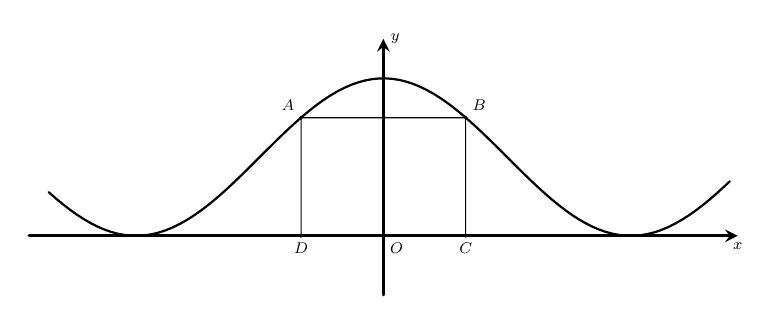
\begin{tikzpicture}[scale=0.5,>=stealth, font=\footnotesize, line join=round, line cap=round]
			\tikzset{every node/.style={scale=0.7}}
			\draw[->,line width=1pt] (-9,0)--(9,0) node[below]{$x$};
			\draw[->,line width=1pt] (0,-1.5)--(0,5) node[right]{$y$};
			\draw[thick, domain=-8.5:8.8, samples=100] plot(\x,{2*cos(((\x)/2)*180/pi)+2});
			\draw[fill=black] 
			(0,0) node[below right]{$O$}circle(1pt);
			\draw (-2.09,0)node[below]{$D$}circle(1pt)--(-2.09,3)node[above left]{$A$}circle(1pt)--(2.09,3)node[above right]{$B$}circle(1pt)--(2.09,0)node[below]{$C$}circle(1pt);
		\end{tikzpicture}
	\end{center}
	Ta có
	\allowdisplaybreaks
	\begin{eqnarray*}
	AD=3 &\Leftrightarrow &2 \cos \dfrac{x}{2}+2=3 \Leftrightarrow \cos \dfrac{x}{2}=\dfrac{1}{2}\\
	&\Leftrightarrow& \cos \dfrac{x}{2}=\cos \dfrac{\pi}{3}\Leftrightarrow\hoac{&x=\dfrac{2 \pi}{3}+k 4 \pi \\&x=\dfrac{-2 \pi}{3}+k 4 \pi}~(k \in \mathbb Z).
\end{eqnarray*}
	Chọn $A\left(\dfrac{-2 \pi}{3}; 3\right)$; $B\left(\dfrac{2 \pi}{3}; 3\right)$; $C\left(\dfrac{2 \pi}{3}; 0\right)$; $D\left(\dfrac{-2 \pi}{3}; 0\right)$.\\
	Khi đó $AB=\dfrac{4 \pi}{3}$; $AD=3$. Vậy $S_{ABCD}=4 \pi \approx 12{,}6~ \left(\mathrm{~m}^{2}\right)$.
}
\end{ex}

\begin{ex}%[1D1V5-2]%[KNTT - Lớp 11 - Ôn tập giữa học kì 1 - Đề 3]%[Phúc Hậu]
	Tính tổng các giá trị nguyên của tham số $m$ để phương trình \hfill\break $m \cos x-m^2-8=2 \cos x-6 m$ có nghiệm.
	\shortans{$14$}
	\loigiai{
	Ta có $m \cos x-m^2-8=2 \cos x-6 m \Leftrightarrow(m-2) \cos x=m^2-6 m+8$.\\
	Trường hợp 1: $m-2=0 \Leftrightarrow m=2$. Khi đó phương trình (1) tương đương với $0 \cdot \cos x=0$ nên phương trình có vô số nghiệm.\\
	Trường hợp 2: $m-2 \neq 0 \Leftrightarrow m \neq 2$. Khi đó phương trình (1) tương đương với
	\[\cos x=\dfrac{m^{2}-6 m+8}{m-2}=m-4.\]
	Phương trình $\cos x=m-4$ có nghiệm khi và chỉ khi $-1 \leq m-4 \leq 1 \Leftrightarrow 3 \leq m \leq 5$.\\
	Do đó phương trình (1) có nghiệm $\Leftrightarrow\hoac{&m=2 \\&m \in[3 ; 5]}$. \\
	Suy ra giá trị nguyên của $m$ thỏa mãn là $2 ; 3 ; 4 ; 5$.\\
	Vậy tổng các giá trị nguyên của tham số $m$ là $14$.
}
\end{ex}

\begin{ex}%[1D2V3-8]%[KNTT - Lớp 11 - Ôn tập giữa học kì 1 - Đề 3]%[Phúc Hậu]
	Nghiên cứu cho thấy rằng nguy cơ tử vong do thuốc lá tăng $2 \%$ mỗi năm ở những người hút thuốc nghĩa là sau $n$ năm, nguy cơ tử vong do hút thuốc theo độ tuổi được tính theo công thức $D_{n}=D_{0}\cdot(1+0{,}02)^{n}$, trong đó $D_{0}$ là nguy cơ tử vong ban đầu của người hút thuốc. Nếu nguy cơ ban đầu ở tuổi 30 là $10 \%$ thì nguy cơ tử vong do hút thuốc khi người này 60 tuổi là $a \%$ ($a$ được làm tròn kết quả đến hàng phần mười). Tìm $a$.
	\shortans{$18{,}1$}
	\loigiai{
	Ta có $D_0=10$. Từ năm 30 tuổi, sau $60-30=30$ năm nữa thì người đó $60$ tuổi.\\
	Vậy đến năm 60 tuổi, nguy cơ tử vong do hút thuốc của người này là
	\[D=10(1+0,02)^{30}\approx 18{,}1(\%).\]
}
\end{ex}

\begin{ex}%[1H4V1-4]%[KNTT - Lớp 11 - Ôn tập giữa học kì 1 - Đề 3]%[Phúc Hậu]
	Cho tứ diện $ABCD$. Trên cạnh $AC$, $AD$ lấy lần lượt các điểm $M$, $N$ sao cho $AM=\dfrac{1}{3}AC$, $AN=2ND$. Gọi $I$ là giao điểm của đường thẳng $MN$ và mặt phẳng $(BCD)$. Biết tỉ số $\dfrac{ID}{IC}=\dfrac{a}{b}$ với $\dfrac{a}{b}$ là phân số tối giản. Giá trị $a+2 b$ bằng bao nhiêu?
	\shortans{$9$}
	\loigiai{
	\immini{Gọi $I$ là giao điểm của đường thẳng $MN$ và $CD$.\\
	Khi đó $\heva{&I \in MN \\&I \in CD \subset(BCD)} \Rightarrow MN \cap(BCD)=\{I\}$.\\
	Kẻ $DE \parallel AC,\, (E \in I M)$.\\
	Do $DE \parallel CM$ nên $\dfrac{ID}{IC}=\dfrac{ED}{MC}\Rightarrow \dfrac{ID}{IC}=\dfrac{ED}{2AM}$.\\
	Do $DE \parallel AM$ nên $\dfrac{ED}{AM}=\dfrac{ND}{NA}=\dfrac{1}{2}$.\\
	Từ và ta có $\dfrac{ID}{IC}=\dfrac{1}{4}$.\\
	Vậy $a+2 b=9$.}{\begin{tikzpicture}[scale=1, font=\footnotesize, line join=round, line cap=round, >=stealth]
		\path
		(0,0) coordinate (B)
		(1.5,-1.5) coordinate (C)
		(4,0) coordinate (D)
		(1,3) coordinate (A)
		($(A)!1/3!(C)$) coordinate (M)
		($(A)!2/3!(D)$) coordinate (N)
		(intersection of M--N and C--D) coordinate (I)
		($(M)+(D)-(C)$) coordinate (i)
		(intersection of D--i and N--I) coordinate (E)
		;
		\draw 
		(A)--(B)--(C)--(D)--(A)--(C)
		(M)--(I)--(D)--(E)
		;
		\draw[dashed] 
		(B)--(D) 
		;
		\foreach \p/\g in {B/170, C/-90, D/0, A/90, M/170, N/30, I/-10, E/80}
		\draw[fill=black] (\p) circle (1pt) node[shift=(\g:3mm)] {$\p$};
		\end{tikzpicture}}
}
\end{ex}

\begin{ex}%[1H4V3-5]%[KNTT - Lớp 11 - Ôn tập giữa học kì 1 - Đề 3]%[Phúc Hậu]
	Cho hình chóp tứ giác $S.ABCD$ có đáy là hình vuông cạnh bằng $20$ cm. Gọi $M$ là điểm trên cạnh $SC$ sao cho $CM=3MS$. Mặt phẳng $(\alpha)$ đi qua $M$ song song với $BC$ và $CD$ cắt hình chóp theo một tứ giác có diện tích là bao nhiêu?
	\shortans{$25$}
	\loigiai{
	\immini{Ta có $(\alpha)$ song song với $BC$ và $CD$ mà $A$, $B$, $C$, $D$ dồng phẳng suy ra $(\alpha)\parallel (ABCD)$.\\
	Giả sử $(\alpha)$ cắt các mặt bên $(SBC)$, $(SCD)$, $(SAB)$, $(SDA)$ lần lượt theo các giao tuyến $MN$, $MQ$, $NP$, $PQ$ với $N \in SB$, $P \in SA$, $Q \in SD$, suy ra $(\alpha) \equiv(MNPQ)$.\\
	Khi đó $MN \parallel BC \Rightarrow \dfrac{MN}{BC}=\dfrac{SN}{SB}=\dfrac{SM}{SC}=\dfrac{1}{4}$.\\
	Tương tự, ta có được $\dfrac{NP}{AB}=\dfrac{PQ}{AD}=\dfrac{MQ}{CD}=\dfrac{1}{4}$ và $MNPQ$ là hình vuông.\\
	Suy ra $S_{MNPQ}=\left(\dfrac{1}{4}\right)^2\cdot S_{ABCD}=\dfrac{1}{16}S_{ABCD}=\dfrac{1}{16}\cdot 20^2=25$.}{\begin{tikzpicture}[scale=0.8, line join=round, line cap=round, >=stealth]
		\tikzset{every node/.style={scale=0.8}}
		\path
		(0,0) coordinate (A)
		(-1.5,-1.5) coordinate (B)
		(4,0) coordinate (D)
		($(B)+(D)-(A)$) coordinate (C)
		(0.5,3) coordinate (S)
		($(S)!0.25!(C)$) coordinate (M)
		($(S)!0.25!(B)$) coordinate (N)
		($(S)!0.25!(D)$) coordinate (Q)
		($(S)!0.25!(A)$) coordinate (P)
		;
		\draw 
		(S)--(B)--(C)--(D)--(S)--(C) (N)--(M)--(Q)
		;
		\draw[dashed] 
		(S)--(A)
		(B)--(A)--(D) (N)--(P)--(Q)
		;
		\foreach \p/\g in {A/170, B/-90, C/-90, D/0, S/90, M/-119, N/180, Q/20, P/-50}
		\draw[fill=black] (\p) circle (1pt) node[shift=(\g:3mm)] {$\p$};
		%	\pic[draw,angle radius=2mm]{angle=A--H--O};
		\end{tikzpicture}}
}
\end{ex}
\Closesolutionfile{ans}

\indapan{6}{ans-KQ}